\chapter{Cenni di teoria degli insiemi}
Per rappresentare un insieme abbiamo tre possibilità:

\begin{enumerate}
	\item Rappresentazione estensive $A=[0,1,2,3,4]$
	\item Rappresentazione intensiva $A=[x|x\in N\,\text{e}\, x<5]$
	\item Rappresentazione con diagrammi di \textit{Eulero - Venn}:
\end{enumerate}

	\begin{center}
		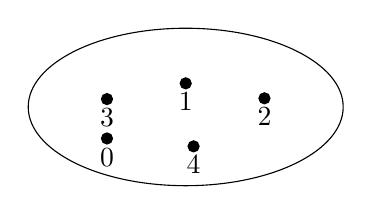
\begin{tikzpicture}domain=0:10] 
		 \draw (0,0) ellipse (2cm and 1cm);
    		 \filldraw  (0,0.3) circle (2pt) node[align=left,   below] {1}
    			(1,0.11) circle (2pt) node[align=left,   below] {2}
    			(-1,-0.4) circle (2pt) node[align=left,   below] {0}
    			(-1,0.1) circle (2pt) node[align=left,   below] {3}
    			(0.1,-0.5) circle (2pt) node[align=left,   below] {4};
		\end{tikzpicture}
	\end{center}


\subsection{Operazioni tra gli insiemi}
Un insieme può essere contenuto in un altro:

\begin{center}
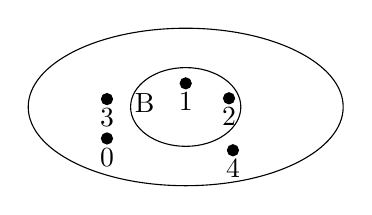
\begin{tikzpicture}domain=0:10] 
    \draw (0,0) ellipse (2cm and 1cm);
     \draw (0,0) ellipse (0.7cm and 0.5cm);

    \filldraw  (0,0.3) circle (2pt) node[align=left,   below] {1}
    (-0.52,0.3) node[align=left,   below] {B}
    (0.55,0.11) circle (2pt) node[align=left,   below] {2}
    (-1,-0.4) circle (2pt) node[align=left,   below] {0}
    (-1,0.1) circle (2pt) node[align=left,   below] {3}
    (0.6,-0.55) circle (2pt) node[align=left,   below] {4};
\end{tikzpicture}
\end{center}

\section{Sottoinsiemi di R}

\subsection{Definizione}

\begin{enumerate}
	\item Un punto $x_0$ si dice intero ad A se esiste un suo interno I($x_0,\delta$)
con $\delta>0$ contenuto in A.
	\item Si dice esterno ad A se è interno al CA ($A^c$).
	\item Si dice di frontiera per A se non è né interno né esterno ad A.
\end{enumerate}
\clearpage

\subsubsection{Interno di A}

\paragraph{°A} Insieme dei punti interni ad A.
\begin{esempio}se $A=(1,3],\text{ }A=(1,3)$\end{esempio}
\paragraph{$\partial$A,FA} Insieme dei punti di frontiera di A
\begin{esempio}se $A=(1,3]$, i punti di frontiera sono i punti $x=1$ e
$x=3$\end{esempio}

\subsubsection{Osservazioni}
\begin{itemize}
	\item Se $x_0\in {^\circ A}\Rightarrow x_0\notin A$
	\item Se $x_0\notin {^\circ A} \text{ (esterno)} \Rightarrow x_0\notin A$
	\item Se $x_0\in\partial A \text{ (frontiera) può essere }x_0\in A \text{
			oppure} x_0 \notin A, \text{ in ogni caso per} \forall
		I(x_0.\delta) $ continue sia punti di A sia punti CA.
\end{itemize}

\begin{defi}
$x_0$ è un punto di accumulazione per A se in $\forall I(x_0,\delta)$ esiste un
punti di A diverso da $x_0$. (Cioè in ogni interno di $x_0 \exists$ infiniti
elementi di A)
	\begin{esempio}
 se $A=(-2,3],x=-2$ è accumulazione per A, ma anche
$x=3,x=0,x=1,\dots$, cioè è di accumulazione per A, qualunque $x\in [2,3]$.\\
DA=A'=derivato di A è l'insieme dei punti di accumulazione per A. Se $x_0\in
DA$ allora può aversi $x_0\in A$ oppure $x_0\notin A$
	\end{esempio}
\end{defi}

\paragraph{Esercizio} $x=1 \text{e} x=3$ sono entrambi punti di accumulazione
per l'intervallo $(1.3],x=3$ appartiene all'intervallo dato, x=1 NO.

\begin{enumerate}
	\item Se $x_0\in A \Rightarrow x_0\in DA$;
	\item Se $x\notin DA$ allora $x_0$ si dice isolato;
	\item Se $DA=\phi\Rightarrow$ A si dice discreto \textbf{Esempio}
		$A=\{1,2,3,4\}$
	\item Se $DA=A\Rightarrow A$ si dice perfetto \textbf{Esempio} $A=[a,b]$
\end{enumerate}
\begin{defi}
Dato $A\subset R$ si definisce chiusura di A e si indica con $\bar{A}$,
l'insieme: $\boxed{\bar{A}=A\bigcup \partial A}$ A è chiuso
$\Leftrightarrow A=\bar{A}$
\end{defi}
\begin{esempio}
	se $A=(2,5]$, allora $\bar{A}=[2,5]$
\end{esempio}

\begin{teorema}
Il teorema di Bolzano Weierstrass afferma che ogni $A\subset R^n$ limitato e
finito possiede almeno un punto di accumulazione. Un insieme chiuso e limitato
in $R^n$ ammette massimo e minimo assoluto.
\end{teorema}
\paragraph{Esempio} $A=[1,4],\text{ } max(A)=4,\text{ } min(A)=1 \text{ }
A=\{x\in R:x^2\leq 1\} \text{ } max{A}=1, \text{ } min(A)=-1$
\clearpage

\section{Funzione di una variabile}
\begin{defi}
Dati A, $B\subseteq R$ una funzione A in B è una legge (o relazione, o mappa)
che ad ogni elemento x di A associa uno ed un solo elemento y di B.
\textit{f}: $A\to B$ oppure $y=f(x)$ $x\in A$ e $y=f(x)\in R$
\begin{itemize}
	\item A = dominio o insieme di definizione di f.
	\item B = codominio di f.
\end{itemize}
Il grafico di $f$ è un insieme di punti del piano (generalmente una curva) che è
sottoinsieme del prodotto cartesiano AxB costituito da (x, f(x)) con $x\in A,
f(x)\in B$
\end{defi}
\begin{defi}
L'immagine di A tramite f, f(A), è l'insieme dei valori di y tale che $\exists
x \in A$ tale che $f(x) \in B$.
	\begin{esempio} Se \textit{f}: $A\to B$ $f(x)=x^2 \text{ } A=R,
	f(A)=[0,+\infty)$\end{esempio}
\end{defi}
\begin{defi}
	Si dice che \textit{f}: $A\to B$
	è suriettiva se $f(A)=B$ (cioè fissato $y\in B \exists x\in A: y=f(x)$)
\end{defi}
\begin{defi}
	Si dice che \textit{f}: $A\to B$ è iniettiva 
	se $x_2\neq x_1\Rightarrow f(x_1) \neq f(x_2)$
\end{defi}
\paragraph{Una funzione può essere sia iniettiva che suriettiva ``biiettiva''}
Se \textit{f} è sia suriettiva che iniettiva allora si dice biiettiva (\textbf{cioè si
ha un corrispondenza biunivoca tra A e B})
\paragraph{Quando una funzione è pari?}
Una funzione è pari se $\forall x\in A: f(x)=f(-x)$ quindi il grafico di
\textit{f} è simmetrico rispetto all'asse Y (es. $y=x^2$)
\paragraph{Quando una funzione è dispari?}
Una funzione è dispari se $\forall x\in A: f(-x)=-f(-x), f(x)=-f(-x)$ quindi il
grafico di \textit{f} è simmetrico rispetto all'origine (es. $y=x^3$)
\paragraph{Quando una funzione è periodica?}
Una funzione $A\to B$ è periodica di periodo $T>0$, se $\forall x \in A, x+T\in
A \text{ e } f(x+T)=f(x)$ 
\subparagraph{Esempio} Funzioni trigonometriche
\paragraph{Quando una funzione è limitata superiormente?}
Una funzione si dice limitata superiormente se $\exists M\in R: f(x)\leq M$
$\forall x \in A$ (il grafico di \textit{f} sta sotto la retta orizzontale $y=m$)
\paragraph{Quando una funzione è limitata inferiormente?}
Analogamente, al caso precedente, una funzione si dice limitata inferiormente
se $\exists m\in R:f(x)\leq m \forall x \in A$ (il grafico di \textit{f} sta
sopra la retta orizzontale $y=m$. La funzione f si dirà limitata se è limitata
sia inferiormente che superiormente).
\paragraph{Quando una funzione viene definita \textit{composta}?}
Una funzione $A\to B \text{ e } B\to C$ si definisce composta di \textit{f} e
\textit{g}: $g(f(x))$ La funzione \textit{h}: $A\to C h=g^of$
\begin{esempio} 
	\textit{f}=$x^2,g(x)=3x+2, \text{ } (A \equiv B \equiv C
	\equiv R) g^of=3x^2+2$
\end{esempio}
\begin{esempio}
	\textit{f}=$x^2,g(x)=3x+2$
\end{esempio}
\clearpage

\begin{figure}[!ht]
	\centering
	\begin{tikzpicture}
		\node[] (pic) at (0,0) {\includegraphics[height=8cm]{img/insiemi funzioni
			composte.pdf}};
	\end{tikzpicture}
	\caption{Grafico di insieme di \textit{f}=$x^2,g(x)=3x+2$}
\end{figure}
\begin{equation}
	\boxed{g^o f=3x^2+2}
\end{equation}
L'operazione di composizione non è commutativa ($g^of\neq f^og$). La
composizione di due funzioni biiettive è biiettiva

\paragraph{Quando una funzione è inversa?}
Date \textit{f}: $A\to B$ biiettiva, si definisce funzione inversa di
\textit{f}: $f^{-1}:_B\to A$ tale che $f^{-1}$ o $f=I_A$ \textit{f} o
$f^{-1}=I_B$

\begin{nota}
	La funzione $y=x^2$ (\textit{f}: $R\to R$) non è biiettiva ma è stata
	''resa'' biiettiva, quindi invertibile, restringendo il suo dominio
	(per l'iniettività) e codominio (per la suriettività). Nell'esempio il
	dominio è stato <<rimpicciolito>> in modo tale da avere una funzione
	strettamente crescente e quindi iniettiva. Il codominio è stata
	<<rimpicciolito>> all'intervallo massimale $[0,+\infty)$ e la funzione è
	diventata anche suriettiva.
\end{nota}
\paragraph{Quando una funzione viene definita monotona?}
Sia \textit{f}:$A\to B$, f si dice monotona in A se verifica una delle seguenti
condizioni ($\forall x_1,x_2\in A$)

\begin{enumerate}
	\item \textit{f} strettamente crescente se $x_1<x_2$, $f(x_1)<f(x_2)$
	\item \textit{f} crescente se $x_1<x_2$, $f(x_1)\leq f(x_2)$
	\item \textit{f} strettamente decrescente se $x_1<x_2$, $f(x_1)<f(x_2)$
	\item \textit{f} decrescente se $x_1<x_2$, $f(x_1)\geq f(x_2)$
\end{enumerate}
\fbox{
 	\addtolength{\linewidth}{-2\fboxsep}%
 	\addtolength{\linewidth}{-2\fboxrule}%
 	\begin{minipage}{\linewidth}
		\textit{Se si verificano la 1 e 3 allora la funzione f(x) è {\color{red}
			strettamente monotona.}}
		\begin{teorema}
			Una funzione $f : A \to B $ strettamente monotona in A, è
			invertibile in A. Inoltre la sua inversa è ancora strettamente
			monotona.
		\end{teorema}
	\end{minipage}
}
\clearpage
